% !TeX spellcheck = en_GB
% Template created by Karol Kozioł (www.karol-koziol.net) for ShareLaTeX

\documentclass[a4paper,9pt]{extarticle}
\usepackage[utf8]{inputenc}
\usepackage[T1]{fontenc}
\usepackage{graphicx}
\usepackage[x11names]{xcolor}
\usepackage{tikz}
\usepackage{fontawesome5}
\usepackage{bm}
\usepackage[most]{tcolorbox}
\usepackage{enumerate}
\usepackage[shortlabels]{enumitem}
\tcbuselibrary{skins,raster,theorems,breakable}

\usepackage{amsmath,amssymb,textcomp}
\usepackage{mathtools}
\everymath{\displaystyle}
\usepackage{multicol}
\usepackage{multirow}
\setlength{\columnseprule}{0pt}
\setlength{\columnsep}{20.0pt}


\usepackage{geometry}
\geometry{a4paper,left=10mm,right=10mm,top=10mm,bottom=15mm}

\newcommand{\trans}[1]{{#1}^{\mathsf{T}}}
\newcommand{\ev}[1]{\mathbb{E}\left[#1\right]}
\newcommand{\unmezz}{\frac{1}{2}}

\newtcolorbox{riquadro}[1][]{enhanced, breakable,frame style={top color=Aquamarine3,bottom color=Aquamarine3},colback=black!80,coltext=Aquamarine3!50,title=#1,fonttitle=\bfseries,halign title=center,coltitle=black!80}
\makeatletter
\renewcommand*{\maketitle}{%
	\noindent
	\begin{minipage}{0.4\textwidth}
		
\begin{tikzpicture}
			\node[rectangle,rounded corners=6pt,inner sep=10pt,fill=SteelBlue4,text width= 0.95\textwidth] {\color{white}\Huge \@title};
		\end{tikzpicture}
	\end{minipage}
	\hfill
	\begin{minipage}{0.55\textwidth}
		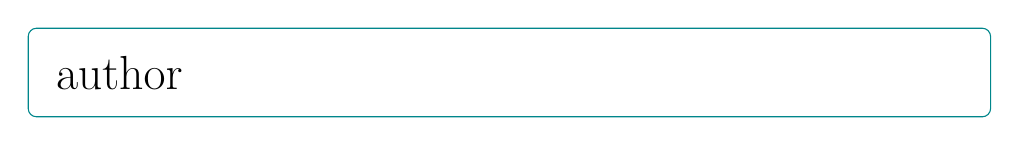
\begin{tikzpicture}
			\node[rectangle,rounded corners=3pt,inner sep=10pt,draw=Turquoise4,text width= 0.95\textwidth] {\LARGE \@author};
		\end{tikzpicture}
	\end{minipage}
}%
\makeatother
\newtcbtheorem[number within=section]{myproof}{Proof}{
	enhanced, sharp corners, breakable,
	colframe=LightSalmon1, coltitle=black, colbacktitle=gray!24,
	coltext=LightSalmon1!60,
	colback=black!80,
	rounded corners,
	fonttitle=\bfseries,
	separator sign={:},
	theorem hanging indent/.try=0pt,
}{ciao}

% custom section
\usepackage[explicit]{titlesec}
\newcommand*\sectionlabel{}
\newcommand{\pr}{\mathbb{P}}
\newcommand{\mbf}[1]{\mathbf{#1}}

\titleformat{\section}
{\gdef\sectionlabel{}
	\normalfont\rmfamily\Large\bfseries}
{\gdef\sectionlabel{\thesection\ }}{0pt}
{
	\noindent
	\begin{tikzpicture}
		\node[rectangle,rounded corners=3pt,inner sep=4pt,fill=Turquoise4,text width= 0.95\columnwidth] {\color{white}\sectionlabel#1};
	\end{tikzpicture}
}
\titlespacing*{\section}{0pt}{0pt}{-10pt}
\newcommand*\subsectionlabel{}
\titleformat{\subsection}
{\gdef\subsectionlabel{}
	\normalfont\rmfamily\Large\bfseries}
{\gdef\subsectionlabel{\thesubsection\ }}{0pt}
{
	\noindent
	\begin{tikzpicture}
		\node[rectangle,inner sep=4pt,fill=Turquoise4!60!black,rounded corners=3pt,text width= 0.9\columnwidth] {\color{white}\subsectionlabel#1};
	\end{tikzpicture}
}
\titlespacing*{\subsection}{0pt}{0pt}{0pt}

% custom footer
\usepackage{fancyhdr}
\makeatletter
\pagestyle{fancy}
\fancyhead{}
\fancyfoot[C]{\footnotesize \textcopyright\ \@date\ \ \@author}
\renewcommand{\headrulewidth}{0pt}
\renewcommand{\footrulewidth}{0pt}
\makeatother

\usepackage{utfsym}

\title{Complex Networks Cheatsheet}
\author{\usym{1F3BC}\;Kotatsu, the Bringer of Jazz\;\usym{1F3B9}}
\date{\today}



\begin{document}
	
	\maketitle
	
	\begin{multicols*}{2}
	\section{General networks}
	Maximum number of links:
	\begin{equation*}
		L_{\max}={N\choose2}=\frac{N(N-1)}{2}.
	\end{equation*}
	Density:
	\begin{equation*}
		d=\frac{L}{L_{\max}}=\frac{2L}{N(N-1)}.
	\end{equation*}
	If $d\ll 1$ then the network is sparse.
	Degree:
	\begin{equation*}
		k_{i}=|N_{i}|.
	\end{equation*}
	Strength: weighted degree
	\begin{equation*}
		s_{i}=\sum_{j\in N_{i}}w_{ij}.
	\end{equation*}
	\begin{riquadro}[Average degree]
		\begin{align*}
		\ang{k}&=\frac{\sum_{i\in N}^{k_{i}}}{N}\\
		&=\frac{2L}{N}\\
		&=\frac{dN(N-1)}{N}\\
		&=d(N-1).
	\end{align*}
	\end{riquadro}
	The average degree is also connected to density:
	\begin{equation*}
		d=\frac{\ang{k}}{N-1}=\frac{\ang{k}}{k_{\max}}.
	\end{equation*}
	\begin{riquadro}[Average path length]
		\begin{equation*}
		\ang{l}=\frac{\sum_{ij}l_{ij}}{N(N-1)}.
	\end{equation*}
	\end{riquadro}
	Diameter of the graph:
	\begin{equation*}
		l_{\max}=\max_{i,j}l_{ij}.
	\end{equation*}
	Trick to avoid this bitch to go towards infinity:
	\begin{equation*}
		\ang{l}=\left(\frac{\sum_{ij}\frac{1}{l_{ij}}}{N(N-1)}\right)^{-1}.
	\end{equation*}
	\begin{riquadro}[Breadth-first search]
		Hold the frontier in a FIFO queue, which initially holds the frontier. All nodes have distance $\ell=-1$ except for $\ell(\text{source})=1$. Initialize the shortest path tree with all nodes and no links. Until the frontier is empty:
		\begin{enumerate}
			\item remove next node $i$ in frontier;
			\item for each neighbour $j$ of $i$ with $\ell(j)=-1$:
			\begin{enumerate}
				\item queue $j$ into frontier;
				\item $\ell(j)=\ell(i)+1$;
				\item add link $(i\to j)$ to shortest path tree.
			\end{enumerate}
		\end{enumerate}
	\end{riquadro}
	We say that the average path length is short (``small world'') when it is about
	\begin{equation*}
		\ang{l}\approx \log N.
	\end{equation*}
	\section{Strong and weak ties}
	\subsection{Triadic closure}
	\begin{riquadro}[Clustering coefficient]
		$$C_{t}(i)=\frac{2\tau(i)}{k_{i}(k_{i}-1)}.$$
		High: friendship transitivity, low: compare with random graph (edges reshuffled).
	\end{riquadro}
	We say that an edge joining two nodes $A$ and $B$ in a graph is a bridge if deleting the edge
	would cause $A$ and $B$ to lie in two different components.\\
	We say that an edge joining two nodes $A$ and $B$ in a graph is a local bridge if its
	endpoints $A$ and $B$ have no friends in common — in other words, if deleting the edge
	would increase the distance between $A$ and $B$ to a value $> 2$. The span is the distance its endpoints would be from each other if the edge was deleted.
	\begin{riquadro}[Neighbourhood Overlap]
		\begin{equation*}
			O_{AB}=\frac{|N(A)\cap N(B)|}{|N(A)\cup N(B)|}
		\end{equation*}
		(without counting $A$ or $B$).
	\end{riquadro}
	\begin{equation*}
		O_{AB}=0\iff(A,B)\text{ is a local bridge}.
	\end{equation*}
	Embeddedness: $|N(A)\cap N(B)|$.
	\subsection{Structural holes}
	Benefits:
	\begin{itemize}
		\item informational advantage;
		\item creativity;
		\item gatekeeping;
		\item may be fucked by triadic closure.
	\end{itemize}
	\section{Homophily}
	\begin{riquadro}[Homophily test]
		Signal of Homophiliy: check if 
		\begin{equation*}
			\#\text{ of cross group edges}<2pq
		\end{equation*}
		and if it is significantly less then there is a strong signal of homophily.
	\end{riquadro}
	The average of $i$'s neighbours' degrees is
	\begin{equation*}
		k_{nn}(i)=\frac{1}{k_{i}}\sum_{j}a_{ij}k_{j};
	\end{equation*}
	with a little abuse of notation define the \textbf{degree correlation function} as the average of all the $k_{nn}\left(k_{i}\right)$ for all nodes whose degree is $k$.
	\begin{riquadro}[Degree correlation function]
		\begin{equation*}
			k_{nn}(k)={\ang{k_{nn}(i)}}_{i:k_{i}=k}.
		\end{equation*}
	\end{riquadro}
	This is the average of all the neighbours' degree of $k$-degree nodes.
	Closures with foci:
	\begin{itemize}
		\item triadic closure (friendship transitivity);
		\item focal closure (selection);
		\item membership closure (influence).
	\end{itemize}
	\section{Centrality measures}
	Average degree of the network:
	\begin{equation*}
		\ang{k}=\frac{\sum_{i}k_{i}}{N}=\frac{2L}{N}
	\end{equation*}
	\begin{riquadro}[Closeness]
		\begin{equation*}
			g_{i}=\frac{1}{\sum_{j\neq i}\ell_{ij}}
		\end{equation*}
		where $\ell_{ij}$ is the distance between nodes $i$ and $j$.
	\end{riquadro}
	A node is the more central the closer it is to the other nodes, on average.
		\begin{riquadro}[Betweenness]
		\begin{equation*}
			b_{i}=\sum_{h\neq j\neq i}\frac{\sigma_{hj}(i)}{\sigma_{hj}}.
		\end{equation*}
		If $n_{k}$ is the number of nodes with degree $k$ then $f_{k}=\frac{n_{k}}{N}$ is the frequency of degree $k$.
	\end{riquadro}
	\begin{riquadro}[Heterogeneity parameter]
		\begin{equation*}
			\kappa=\frac{\ang{k^{2}}}{\ang{k}^{2}}
		\end{equation*}
		with
		\begin{equation*}
			\ang{k}=\frac{\sum_{i}k_{i}}{N}\qquad\ang{k^{2}}=\frac{\sum_{i}k^{2}_{i}}{N}
		\end{equation*}
		\end{riquadro}
		if most degrees have the same value $k_{0}$
		\begin{equation*}
			\ang{k}\approx k_{0},\quad\ang{k^{2}}\approx k_{0}^{2}\implies \kappa\approx1
		\end{equation*}
		and we have $\kappa\gg1$ if the distribution is very heterogeneous 
\section{Network models}
\begin{riquadro}[Power law distribution]
	\begin{equation*}
		f(k)=ak^{-c}
	\end{equation*}
\end{riquadro}
	The network is \textbf{scale free} with $2<c<3$ when $N\to\infty\implies \ang{k^{2}\to\infty}$. We can approximate with a straight line
\begin{equation*}
	y=\log a-cx.
\end{equation*}
\begin{riquadro}[RichGetRicher process]
	\begin{enumerate}
		\item Nodes are created in a sequence $1,2,\ldots,N$.
		\item For each node $j$ that joins the network:
		\begin{itemize}
			\item w.p. $p$ page $i$ is selected uniformly at random and a link $(j,i)$ is created;
			\item w.p. $1-p$ page $i$ is selected uniformly at random, $l$ is the page $i$ is connected to, then a link $(j,l)$ is created.
		\end{itemize}
	\end{enumerate}
\end{riquadro}
Connection between Zipf's law, Pareto's law and power law:
\begin{itemize}
	\item Zipf: $k\approx j^{-b}$;
	\item Pareto: $\pr(K>k)\approx k^{-y}$;
	\item Power law: $f(k)\approx k^{-c}$.
\end{itemize}
It is possible to prove that 
\begin{equation*}
	c=1+\gamma\qquad\gamma=\frac{1}{b}.
\end{equation*}
\section{Models of networks}
\subsection{Random networks}
Most real world networks have low average path length.
\begin{riquadro}[Gilbert random network model]
	\begin{enumerate}
		\item Start with $N$ nodes and zero links.
		\item Go over all pairs of nodes. For each pair of nodes $i$ and $j$ toss the coin and decide whether to connect $i$ and $j$.
	\end{enumerate}
\end{riquadro}
Expected number of links $\ang{L}$ of a random network with $N$ nodes:
\begin{equation*}
	\ang{L}=p\frac{N(N-1)}{2}.
\end{equation*}
Expected density of links $d$ of a random network:
\begin{equation*}
	d=\frac{\ang{L}}{\frac{N(N-1)}{2}}=\frac{\frac{pN(N-1)}{2}}{\frac{N(N-1)}{2}}=p
\end{equation*}
Expected average degree: it is the number of heads with probability of yielding heads equal to $p$ and $t$ trials equal to the number of potential neighbours of a node ($t=N-1$):
\begin{equation*}
	\ang{k}=p(N-1).
\end{equation*}
Probability that a node has $k$ neighbours: binomial distribution.
\begin{equation*}
	\pr(k)={N-1\choose k}p^{k}(1-p)^{(N-1)-k}.
\end{equation*}
Since nodes have approximately the same degree $k$, for $k$ large enough the total number of nodes within a distance $d$ is:
\begin{equation*}
	N_{d}\approx k(k-1)^{d}\approx k^{d}.
\end{equation*}
To cover the whole network we need 
\begin{equation*}
	d_{\max}\approx\frac{\log N}{\log k}
\end{equation*}
steps. \\
The probability that two nodes are connected is just the probability $p$ that any two nodes of the graph are connected:
\begin{equation*}
	C_{i}=p=\frac{\ang{k}}{N-1}\approx\frac{\ang{k}}{N}.
\end{equation*}
In general, the average clustering coefficient is lower than on real networks of the same size and average degree (no hubs!).
\subsection{Small world networks}
We seek to build a network with small-world property and high clustering coefficient.
\begin{riquadro}[Watts-Strogatz model]
	We have $N$ nodes forming a regular ring lattice with degree $k$. With probability $p$ rewire a link randomly.
\end{riquadro}
Expected number of rewired links:
\begin{equation*}
	pL=\frac{pNk}{2}.
\end{equation*}
These networks have the high clustering coefficient and have the small world property, but there are no hubs (damn).
\begin{riquadro}[Configuration model]
	Builds networks with a pre-definite degree sequence. We use a list of $N$ numbers $k_{1},\ldots,k_{n}$ where $k_{i}$ is the degree of node $i$. Each node must have as many stubs as its assigned degree, then attach the stubs at random.
\end{riquadro}
Here the randomization preserves the degree.
\subsection{Preferential models networks}
\begin{riquadro}[Network growth]
	\begin{enumerate}
		\item A new node comes with a given number of stubs.
		\item The stubs are attached to some of the old nodes.
	\end{enumerate}
\end{riquadro}
	This features:
\begin{itemize}
	\item growth;
	\item preferential attachment.
\end{itemize}
Example: Polya's urn. 
\begin{riquadro}[Barabàsi-Albert model]
	\begin{enumerate}
		\item Start with $m_{0}$ nodes (usually fully connected).
		\item At each step a new node $i$ is added to the system and sets $m$ links with some of the older nodes ($m\leq m_{0}$).
		\item The probability that the new node $i$ chooses an older node $j$ as neighbour is proportional to the degree $k_{j}$ of $j$:
		\begin{equation*}
			\Pi(i\leftrightarrow j)=\frac{k_{j}}{\sum_lk_l}.
		\end{equation*}
		\item The procedure ends when the given number $N$ of nodes is reached.
	\end{enumerate}
\end{riquadro}
We see that preferential attachment is necessary for the formation of hubs, time alone is not enough.
\section{Power laws}
Recall that the heterogeneity parameter is a measure of the distribution's broadness:
\begin{equation*}
	\kappa=\frac{\ang{k^{2}}}{\ang{k}^{2}}.
\end{equation*} 
As a function of degree $k$, what fraction of nodes has the degree $k$? Empirical findings:
\begin{equation*}
	f(k)\approx k^{-c}
\end{equation*}
\begin{riquadro}[Power law distribution]
	\begin{equation*}
		f(k)=ak^{-c}.
	\end{equation*}
\end{riquadro}
For $2<c<3$ we have that when $N\to\infty$ then $\ang{k}^{2}\to\infty$: \textbf{scale free network}. The distribution is unbounded when $N\to\infty$, with infinite variance. Tails are heavier than we expect so there are pages more popular than expected. \\
We can approximate the power law:
\begin{equation*}
	\begin{array}{c}
		f(k)=ak^{-c}=\log f(k)=\log a+c\log k\\
		\Downarrow\\
		y=\log a-cx.
	\end{array}
\end{equation*}
Power laws are produced by feedback effects: but popularity is a fragile thing. We can predict that a power law can emerge after a while, so we can predict that there will be hubs.\\
Define a r.v. $X_{j}(t)=\#$ of links to $j$ at a time step $t$ with:
\begin{equation*}
	\begin{cases}
		X_{j}(0)=0\\
		X_{j}(t+1)=X_{j}(t)+\frac{p}{t}+\frac{(1-p)X_{j}(t)}{t}.
	\end{cases}
\end{equation*}
Taking the derivative we get
\begin{equation*}
	\frac{\dx_{j}}{\dt}=\frac{p}{t}+\frac{(1-p)x_{j}}{t}=\frac{p+qx_{j}}{t}.
\end{equation*}
So
\begin{align*}
	&\frac{\dx_{j}}{\dt}=\frac{p+qx_{j}}{t}\\
	\implies&\frac{1}{p+qx_{j}}\cdot\frac{\dx_{j}}{\dt}\dt=\frac{1}{t}\dt.
\end{align*}
Integrating both sides yields:
\begin{align*}
	&\int\frac{1}{p+qx_{j}}\cdot\dx_{j}=\int\frac{1}{t}\dt\\
	\implies&q\left(\frac{\ln(p+qx_{j})}{q}+c_{1}\right)=q\left(\ln t+c_{2}\right)\\
	\implies&\ln\left(p+qx_{j}\right)=q\ln t+c.
\end{align*}
Set $A=e^{c}$ and exponentiate both sides"
\begin{align*}
	&p+qx_{j}=At^{q}\\
	\implies&x_{j}(t)=\frac{1}{q}\left(At^{q}-p\right).
\end{align*}
Using the initial condition:
\begin{equation*}
	0=\frac{1}{q}\left(Aj^{q}-p\right)\implies A=\frac{p}{j^{q}}.
\end{equation*}
Substitute and get
\begin{align*}
	x_{j}(t)&=\frac{1}{q}\left(\frac{p}{j^{q}}t^{q}-p\right)\\
	&=\frac{p}{q}\left[{\left(\frac{t}{q}\right)}^{p}-1\right].
\end{align*}
\begin{riquadro}
	\begin{equation*}
		x_{j}(t)=\frac{p}{q}\left[\left(\frac{t}{j}\right)^{q}-1\right]
	\end{equation*}
\end{riquadro}
What fraction of all functions $x_{j}$ satisfies $x_{j}\geq k$ at time $t$?
\begin{equation*}
	x_{j}(t)=\frac{p}{q}\left[\left(\frac{t}{j}\right)^{q}-1\right]\geq k.
\end{equation*}
We can rewrite it in terms of $j$:
\begin{riquadro}
	\begin{equation*}
	j\leq t\left(\frac{q}{p}k+1\right)^{-\frac{1}{q}}.
\end{equation*}
\end{riquadro}
The fraction of values $j$ that satisfy the above inequality is:
\begin{align*}
	F(k)&=\frac{1}{t}\cdot t\left(\frac{q}{p}k+1\right)^{-\frac{1}{q}}\\
	&=\left(\frac{q}{p}k+1\right)^{-\frac{1}{q}}
\end{align*}
so we have a power law:
\begin{equation*}
	F(k)\propto k^{-\frac{1}{q}}.
\end{equation*}
To find $f(k)$ take the derivative:
\begin{align*}
	-\frac{\dif F}{\dif k}&=-\frac{\dif\left(\frac{q}{p}k+1\right)^{-\frac{1}{q}}}{\dif k}\\
	&=\frac{1}{q}\cdot\frac{q}{p}\cdot\left(\frac{q}{p}k+1\right)^{-1-\frac{1}{q}}\\
	&=\frac{1}{q}\cdot\left(\frac{q}{p}k+q\right)^{-1-\frac{1}{q}}\propto k^{-\left(1+\frac{1}{q}\right)}
\end{align*}
which is a power law with exponent
\begin{equation*}
	1+\frac{1}{q}=1+\frac{1}{1-p}.
\end{equation*}
So we have
\begin{equation*}
	\lim_{p\to1}\left(1+\frac{1}{p}\right)=\infty
\end{equation*}
which means that when link formation is governed by random choice large numbers of in-degree are extremely rare and
\begin{equation*}
	\lim_{p\to0}\left(1+\frac{1}{p}\right)=2
\end{equation*}
which means that the growth is mainly governed by preferential attachment.
	\section{Community detection}
	Internal link density for community $C$:
	\begin{align*}
		\delta^{\mathrm{int}}_{C}&=\frac{L_{C}}{L_{C}^{\max}}\\
		&=\frac{L_{C}}{{N_{C}\choose 2}}\\
		&=\frac{2L_{C}}{N_{C}(N_{C}-1)}.
	\end{align*}
		\subsection{Clusterin'}
		\begin{riquadro}[Kernighan-Lin algorithm]
			\begin{enumerate}
				\item Split randomly in two groups $A$ and $B$ of predetermined size $N_{A}$ and $N_{B}$.
				\item Choose each pair of nodes one in $A$ and the other in $B$ and compute the variation in cut size (inter-group links) if you swap them.
				\item The pair with the largest decrease in cut size is swapped and locked.
				\item Rinse and repeat till cut size doesn't decrease no' mo'.
			\end{enumerate}
		\end{riquadro}
		Similarity (structural equivalence):
		\begin{equation*}
			S^{\text{SE}}_{ij}=\frac{\{\text{$\#$ of neighbours of $i$}\}\cap\{\text{$\#$ of neighbours of $j$}\}}{\{\text{$\#$ of neighbours of $i$}\}\cup\{\text{$\#$ of neighbours of $j$}\}}.
		\end{equation*}
		Similarity of two groups:
		\begin{itemize}
			\item \textit{single linkage}: $S_{G_{1}G_{2}}=\max_{i,j}S_{ij}$;
			\item \textit{complete linkage}: $S_{G_{1}G_{2}}=\min_{i,j}S_{ij}$;
			\item \textit{average linkage}: $S_{G_{1}G_{2}}={\langle S_{ij}\rangle}_{ij}$;
		\end{itemize}
		\subsection{Community detection}
		Betweenness of an edge $(i,j)$: \# of shortest paths passing through $(i,j)$.
		\begin{riquadro}[Girvan-Newman method]
			\begin{enumerate}
				\item Calculate betweenness for all edges.
				\item Find the edge with highest betweenness. 
				\item Fuck those edge. If there is a tie, pick a random one.
				\item Recalculate the betweenness of remaining links.
				\item Return components as clusters or repeat until desired number of clusters.
			\end{enumerate}
		\end{riquadro}
		Recall homophily: if $p$ is the fractions of nodes in $A$ and $q$ in $B$ then we have homophily if the \# of cross groups edges $<2pq$. \\
		Modularity of community $C$:
		\begin{equation*}
			Q=\frac{1}{L}\sum_{C}\left(L_{C}-\frac{k^{2}_{C}}{4L}\right)
		\end{equation*} where
		\begin{itemize}
			\item $L$: \# of links of all network;
			\item $L_{C}$: \# of links of community $C$;
			\item $k_{C}$: degree of community $C$;
			\item $\frac{k^{2}_{C}}{4L}$: expected \# of internal links of community $C$.
		\end{itemize}
		For directed networks:
		\begin{equation*}
			Q_{d}=\frac{1}{L}\sum_{C}\left(L_{C}-\frac{k_{C}^{\mathrm{in}}k^{\mathrm{out}}_{C}}{L}\right).
		\end{equation*}
		For weighted networks:
		\begin{equation*}
			Q_{w}=\frac{1}{W}\sum_{C}\left(W_{C}-\frac{s^{2}_{C}}{4W}\right).
		\end{equation*}
		For weighted and directed networks:
		\begin{equation*}
			Q_{wd}=\frac{1}{W}\sum_{C}\left(W_{C}-\frac{s^{\mathrm{in}}_{C}s^{\mathrm{out}}_{C}}{W}\right).
		\end{equation*}
		\begin{riquadro}[Newman's greedy algorithm]
			\begin{enumerate}
				\item Start partition with one node in each community.
				\item Merge the pair of groups of nodes that yield the highest increase/lowest decrease of $Q$.
				\item Continue till all nodes are in the same community.
				\item Pick the partition with largest modularity.
			\end{enumerate}
		\end{riquadro}
		\begin{riquadro}[Louvain's algorithm]
			\begin{enumerate}
				\item Each node is a different community.
				\item Each node is put in the community of the neighbour that yields the largest modularity increase $\Delta Q$ with respect to the current partition. Visit all nodes till you can't improve $Q$ by moving nodes.
				\item Transform the network in a weighted supernetwork where every community becomes a supernode with self loop = \# of internal nodes.
				\item Repeat until no further grouping of clusters can increase modularity.
			\end{enumerate}
		\end{riquadro}
		\begin{riquadro}[Label propagation]
			\begin{enumerate}
				\item Each node is assigned to a different community and is given a different label.
				\item Sweep all the nodes in random order: each node takes the label shared by the majority of its neighbours. Pick a random if tie.
				\item If every node has the majority label of its neighbours stop, otherwise go to step 2.
			\end{enumerate}
		\end{riquadro}
		The probability that a network $G$ is reproduced by the degree-corrected stochastic block model is
		\begin{equation*}
			\mathcal{L}(G|g)=\sum_{r,s=1}^{q}L_{rs}\log\left(\frac{L_{rs}}{k_{r}k_{s}}\right).
		\end{equation*}
		$L_{rs}$: links between group $r$ and $s$, $k_{r}$: degree of group $r$ (sum of degrees of nodes in $r$).
		\begin{riquadro}[Fitting a SBM to a network]
			\begin{enumerate}
				\item Random partition in $q$ clusters;
				\item Move a node from one group to the other and at each step select the move that most increases/least decreases the likelihood (every node can be moved once).
				\item When all the nodes have been moved inspect the partitions through which the system passed from start to end of the procedure in step 2 and select the one with highest likelihood.
				\item The likelihood of two consecutive iteration is the same $\to$ stop.
			\end{enumerate}
		\end{riquadro}
		\subsection{Method evaluation}
		We need the benchmarks.
		\begin{itemize}
		\item \textbf{GN Benchmark}.
		Planted partition model: we have
		\begin{itemize}
			\item $q$ groups of identical size $\frac{N}{q}$;
			\item expected internal degree: $\langle k^{\mathrm{int}}\rangle=p_{\mathrm{int}}\left(\frac{N}{q}-1\right)$;
			\item expected external degree: $\langle k^{\mathrm{ext}}\rangle=p_{\mathrm{ext}}\frac{N}{q}(q-1)$;
			\item expected total degree: $\langle k\rangle=\langle k^{\mathrm{int}}\rangle+\langle k^{\mathrm{ext}}\rangle$.
		\end{itemize}
		For the Girvan-Newman benchmark we choose $N=128$, $q=4$, $\langle k\rangle=16$ so that we have 
		\begin{equation*}
			31p_{\mathrm{int}}+96p_{\mathrm{ext}}=16
		\end{equation*}
		and therefore the probabilities are not independent. As long as $p_{\mathrm{int}}>p_{\mathrm{ext}}\implies \langle k_{\mathrm{ext}}\rangle<12$ we should be able to detect communities, but actually the threshold is 9.
		\item \textbf{LFR Benchmark}. The networks produced have heavy tailed distribution of degree and community size.
		\item \textbf{Actual real benchmarks} like Zacahry's karate club network.
		\end{itemize}
		\begin{riquadro}[Fraction of correctly detected nodes]
			A node is correctly identified if at least half of the other nodes in the detected partition are also in the same community in the benchmark partition.
		\end{riquadro}
		The problem is that if the detected partition has communities obtained by merging two or more groups in the benchmark partition then all the nodes of those clusters are considered WRONG.
		\begin{riquadro}[Normalized mutual information]
			We can use NMI to check how much information is shared between the detected partition and the benchmark partition (that is: similar they are). Values near 1 mean high agreement.
		\end{riquadro}
		If we have two partitions $X$ and $Y$ the probability that a randomly chosen node belongs to cluster $x$ with size $N_{x}$ of partition $X$ is
		\begin{equation*}
			\pr(x)=\frac{N_{x}}{N}
		\end{equation*}
		and the probability that a randomly chosen node belongs to cluster $x$ of a partition $X$ and to cluster $y$ of partition $Y$ is
		\begin{equation*}
			\pr(x,y)=\frac{N_{xy}}{N}
		\end{equation*}
		where $N_{xy}$ is the number of nodes shared by $x$ and $y$. Since the entropy of $X$ is
		\begin{equation*}
			H(X)=-\sum_{x}\pr(x)\log\pr(x)
		\end{equation*}
		and
		\begin{equation*}
			H(X|Y)=\sum_{x,y}\pr(x,y)\log\left(\frac{\pr(y)}{\pr(x,y)}\right)
		\end{equation*}
		the NMI is
		\begin{equation*}
			\mathrm{NMI}(X,Y)=\frac{2H(X)-2H(X|Y)}{H(X)+H(Y)}
		\end{equation*}
		\section{Signed networks}
		\subsection{Structural balance}
		\begin{riquadro}[STRONG Structural Balance Pty]
			A labeled complete graph is balanced if every triangle is balanced.
		\end{riquadro}
		\begin{figure}[H]
			\centering
			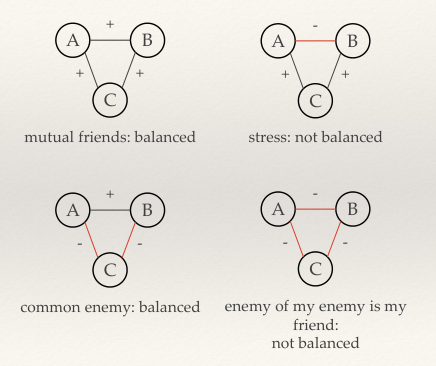
\includegraphics[width=0.7\linewidth]{screenshot001}
			\label{fig:screenshot001}
		\end{figure}
		\begin{riquadro}[Balance Theorem]
			If we can divide the graph in \underline{two} groups where nodes are mutual friends
			inside each group, and enemies are only between nodes in the two groups, then the graph
			is balanced.
		\end{riquadro}
		\begin{riquadro}[WEAK Structural Balance Pty]
			There is no set of three nodes such that the edges among them consist of exactly two
			positive edges and one negative edge
		\end{riquadro}
		\begin{figure}[H]
			\centering
			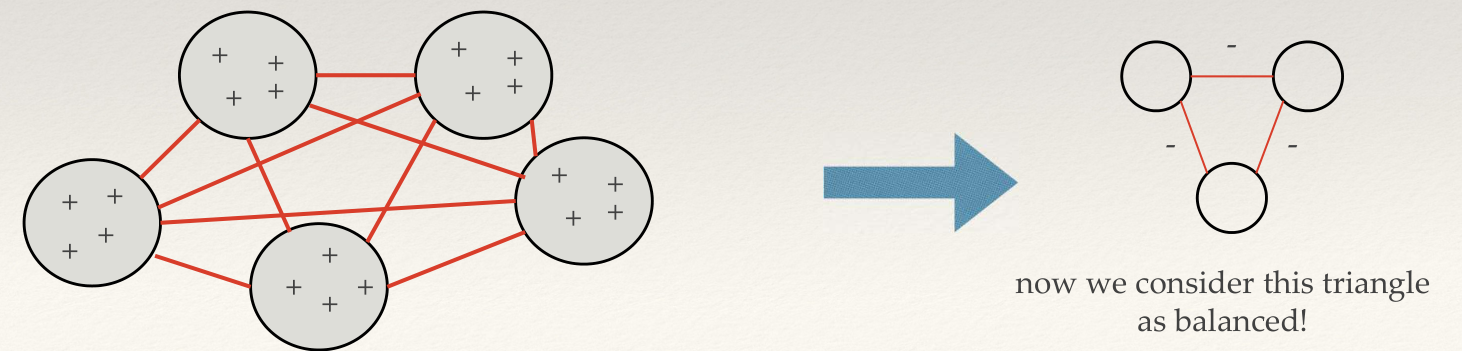
\includegraphics[width=0.7\linewidth]{screenshot002}
			\label{fig:screenshot002}
		\end{figure}
		\begin{riquadro}[WEAK Balance Theorem]
			If a labelled complete graph
			is weakly balanced, then its nodes can be divided into groups in such a way that every
			two nodes belonging to the same group are friends, and every two nodes belonging to
			different groups are enemies.
		\end{riquadro}
		The important difference with the strong theorem is that the strong theorem only allows 2 groups.
		\begin{riquadro}[Arbitrary non complete graphs]
			A signed graph is balanced iff it contains no cycle with an odd number of
			negative edges.
		\end{riquadro}
		We need to 
		\begin{enumerate}
			\item Convert the graphs to a reduced form with only negative edges;
			\item Solve the problem in the reduced graph.
		\end{enumerate}
		\section{Directed networks}
		\subsection{Crawlers}
		\begin{figure}[H]
			\centering
			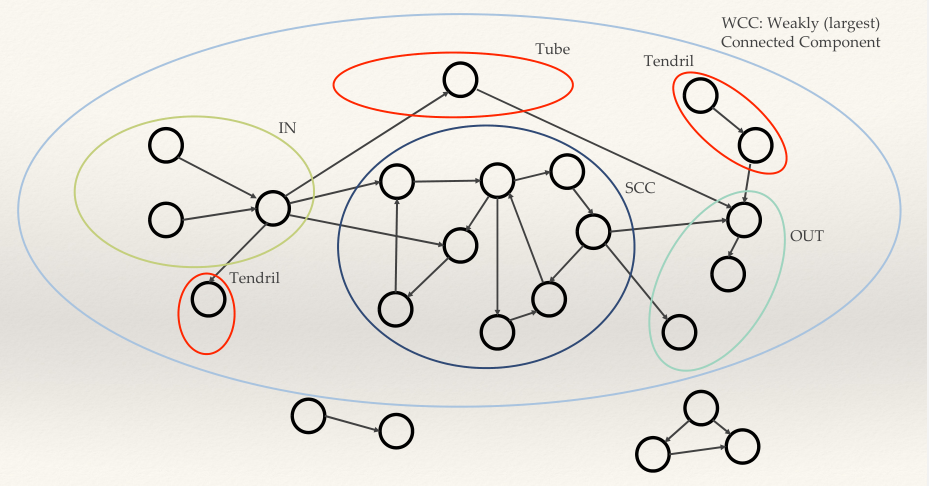
\includegraphics[width=0.7\linewidth]{screenshot003}
			\label{fig:screenshot003}
		\end{figure}
		The Weakly Connected components is made by:
		\begin{itemize}
			\item SCC: largest connected subgraph such that I can find paths leading from a node to another and back;
			\item IN: for every node in here there is a path to the SCC;
			\item OUT: for every node in the SCC there is a path for every node in here, no way back
			\item Tendrils: nodes reachable from IN or nodes that reach OUT (outside of SCC);
			\item Tubes: nodes reached from IN and reaching OUT without being in the SCC.
		\end{itemize}
		\begin{riquadro}[Web Crawler]
			\begin{enumerate}
				\item Start from a set of high-quality seed URLs;
				\item The queue of unvisited URLs is called frontier;
				\item Fetch pages dequeued from the frontier, extract links and add them to the frontiers.
			\end{enumerate}
			Crawlers use \textbf{BFS} because of topical
			locality, to target good-quality
			pages linked by other good-quality
			pages
		\end{riquadro}
		We need more than one seed page, but at least one of these seeds but be in the IN.\\
		For in-degree distribution we have heavy tails with huge hubs:
		\begin{equation*}
			\langle k_{\mathrm{in}}\rangle\sim10,\qquad\kappa\sim40.
		\end{equation*}
		For out-degree distribution we have less meaningfulness, since it depends on individual content providers. The core has the following number of short paths:
		\begin{equation*}
			N\sim1.8\cdot10^{9},\qquad\langle\ell\rangle\sim13.
		\end{equation*}
		\subsection{Cosine similarity}
		The textual content of each page is represented as a one-hot encoding vector
		\begin{equation*}
			\vec{d}=\left\{w_{d,1},\ldots,w_{d,n}\right\}.
		\end{equation*}
		So we remove stop words, we create a vocabulary and calculate the vector for each document. Remember the euclidean dot product
		\begin{equation*}
			\vec{d_{1}}\cdot\vec{d_{2}}=\lVert\vec{d_{1}}\rVert\cdot\lVert\vec{d_{2}}\rVert\cdot\cos\vartheta
		\end{equation*}
		\begin{riquadro}[Cosine similarity]
			\begin{align*}
				\mathrm{sim}\left(\vec{d_{1}},\vec{d_{2}}\right)&=\cos\vartheta\\	
				&=\frac{\vec{d_{1}}\cdot\vec{d_{2}}}{\lVert\vec{d_{1}}\rVert\cdot\lVert\vec{d_{2}}\rVert}\\
				&=\frac{\sum_{t}w_{d_{1},t}\cdot w_{d_{2},t}}{\sqrt{\sum_{t}w^{2}_{d_{1},t}}\cdot\sqrt{\sum_{t}w^{2}_{d_{2},t}}}\in[-1,1]
			\end{align*}
		\end{riquadro}
		\begin{riquadro}[Pearson similarity]
				\begin{equation*}
				r\left(\vec{d_{1}},\vec{d_{2}}\right)=\frac{\sum_{t}\left(w_{d_{1},t}-\overline{w}_{d_{1}}\right)\cdot\left(w_{d_{2},t}-\overline{w}_{d_{2}}\right)}{\sqrt{\sum_{t}\left(w_{d_{1},t}-\overline{w}_{d_{1}}\right)^{2}}\cdot\sqrt{\sum_{t}\left(w_{d_{2},t}-\overline{w}_{d_{2}}\right)^{2}}}
			\end{equation*}
		\end{riquadro}
		\subsection{Network backbone}
		Set a different threshold for each
		node, so that we remove links with weights
		that are not significant compared to the other
		links of that node. Compare the probability of link weight $w_{ij}$ given degree $k_{i}$ and strength $s_{i}$ of node $i$ (normalized weight $\frac{w_{ij}}{s_{i}}$ in interval $[0,1]$) to a significance threshold: keep links if
		\begin{equation*}
			p_{ij}=\left(1-\frac{w_{ij}}{s_{i}}\right)^{k_{i}-1}\leq\alpha.
		\end{equation*}
		This is the probability that a normalized weight equal to or higher than $\frac{w_{ij}}{s_{i}}$ can be obtained by a purely random model. The higher the normalized weight, the lower the probability that this large normalized value could be obtained by pure change. Hence it has to be included in the network backbone.
		\subsection{Authority}
		If we select documents on a given topic the ``in links'' are a measure of authority of a page on such a topic.
		\begin{riquadro}[Hubs and authorities]
			\begin{enumerate}
				\item[Step 0:] Every node has both a hub and an \textit{authority} value initialized to 1.
				\item[Step $k$:] \begin{enumerate}
					\item authorities are updated after $k-1$'s hub values;
					\item hubs are updated on new authority values;
					\item normalize hub and authority values.
				\end{enumerate}
			\end{enumerate}
		\end{riquadro}
		We are interested in the limiting values for hubs and authorities as properties of the link structure.
		\subsection{Spectral Analysis of HITS}
		The adjacency matrix for nodes $1,\ldots,n$ is a $n\times n$ matrix $\mathbf{M}$ with
		\begin{equation*}
			M_{ij}=\begin{cases}
				1&\text{if $(i,j)$ is an edge}\\
				0&\text{otherwise}.
			\end{cases}
		\end{equation*}
		\begin{figure}[H]
			\centering
			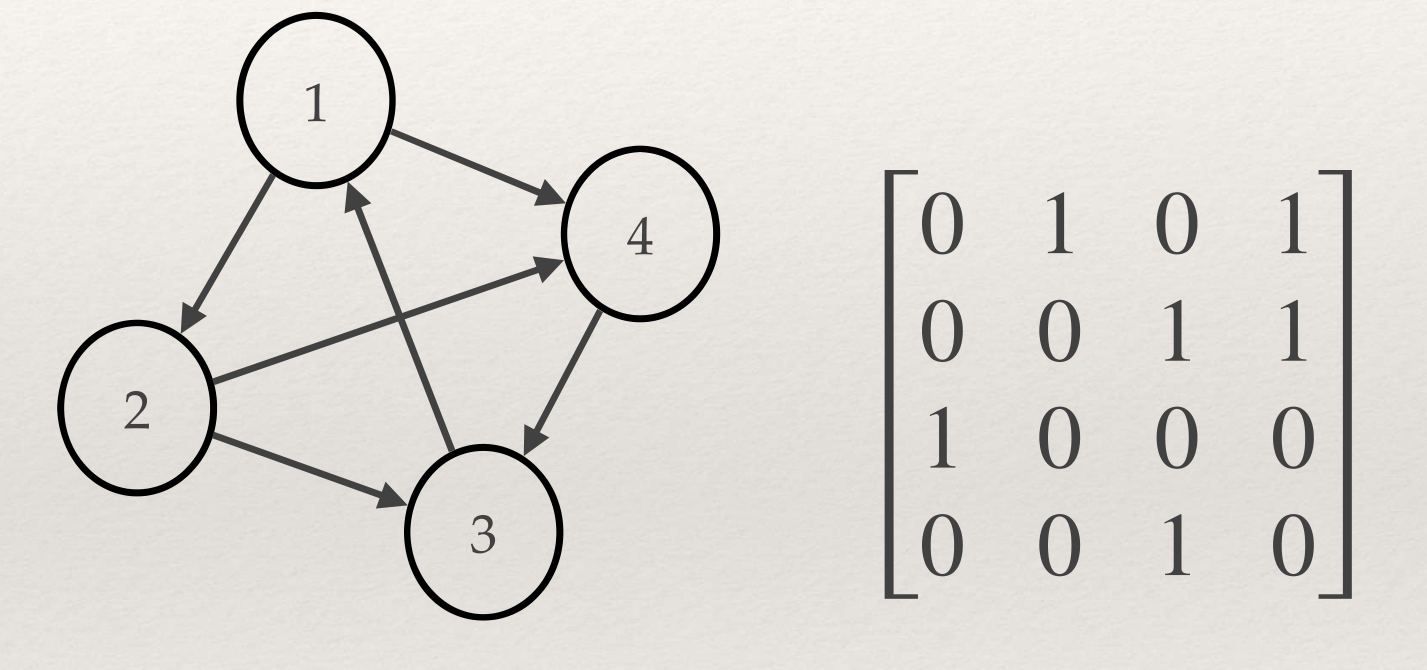
\includegraphics[width=0.7\linewidth]{screenshot004}
			\label{fig:screenshot004}
		\end{figure}
		If $\mathbf{h}$ and $\mathbf{a}$ are $n$-dimensional vectors (respectively hub and authorities values):
		\begin{itemize}
			\item Hub update rule:
			\begin{align*}
				h_{i}&\leftarrow\sum_{j=1}^{n}M_{ij}a_{j}\\
				&=M_{i1}a_{1}+M_{i2}a_{2}+\ldots+M_{in}a_{n}\\
				\mathbf{h}&\leftarrow\mathbf{M}\cdot\mathbf{a}.
			\end{align*}
			\item Authority update rule:
			\begin{align*}
				a_{i}&\leftarrow\sum_{j=1}^{n}M_{ij}h_{j}\\
				\mathbf{a}&\leftarrow\trans{\mathbf{M}}\cdot\mathbf{h}.
			\end{align*}
		\end{itemize}
		After initializing $\mathbf{h}^{<0>}=\underbrace{(1,1,\ldots,1)}_{n}$ after $k$ applications we have
		\begin{align*}
			\mathbf{a}^{<k>}&=\trans{\mathbf{M}}\left(\mathbf{M}\trans{\mathbf{M}}\right)^{k-1}\mathbf{h}^{<0>}\\
			\mathbf{h}^{<k>}&=\left(\mathbf{M}\trans{\mathbf{M}}\right)^{k}\mathbf{h}^{<0>}.
		\end{align*}
		We want to prove that for constants $c$ and $d$ then $\frac{\mathbf{h}^{<k>}}{c^{k}}$ and $\frac{\mathbf{a}^{<k>}}{d^{k}}$ converge for $k\to\infty$. Since $\frac{\mathbf{h}^{<k>}}{c^{k}}=\frac{\left(\mathbf{M}\trans{\mathbf{M}}\right)^{k}\mathbf{h}^{<0>}}{c^{k}}$ converges to $\mathbf{h}^{<\star>}$ then I expect that
		\begin{equation*}
			c\cdot\mathbf{h}^{<\star>}=\left(\mathbf{M}\trans{\mathbf{M}}\right)\cdot\mathbf{h}^{<\star>}.
		\end{equation*}
		But this means that we need to prove that the sequence of $\frac{\mathbf{h}^{<k>}}{c^{k}}$ converges to the eigenvectors of $\mathbf{M}\trans{\mathbf{M}}$.
		Since $\mathbf{M}\trans{\mathbf{M}}$ is symmetric, there exist $n$ eigenvectors $\mathbf{z}_{1},\ldots,\mathbf{z}_{n}$ orthogonal and all unit (they are basis for the space $\R^{n}$). So we can find
		\begin{itemize}
			\item $n$ mutual orthogonal eigenvectors $\mathbf{z}_{1},\ldots,\mathbf{z}_{n}$ (the spectrum of $\mathbf{M}\trans{\mathbf{M}}$);
			\item $n$ corresponding eigenvalues $c_{1},\ldots,c_{n}$.
		\end{itemize}
		We can sort the eigenvectors such that the corresponding eigenvalues are increasing and suppose $c_1$ strictly greater than $c_{2}$. Consider $\mathbf{x}\in\R^{n}$:
		\begin{equation*}
			\mathbf{x}=p_{1}\mathbf{z}_{1}+\ldots+p_{n}\mathbf{z}_{n}
		\end{equation*}
		and
		\begin{align*}
			\left(\mathbf{M}\trans{\mathbf{M}}\right)\mathbf{x}&=\left(\mathbf{M}\trans{\mathbf{M}}\right)\cdot\left(p_{1}\mathbf{z}_{1}+\ldots+p_{n}\mathbf{z}_{n}\right)\\
		&=p_{1}	\left(\mathbf{M}\trans{\mathbf{M}}\right)\mathbf{z}_{1}+\ldots+p_{n}	\left(\mathbf{M}\trans{\mathbf{M}}\right)\mathbf{z}_{n}\\
		&=p_{1}c_{1}\mathbf{z}_{1}+\ldots+p_{n}c_{n}\mathbf{z}_{n}.
		\end{align*}
		So we can say
		\begin{equation*}
			\left(\mathbf{M}\trans{\mathbf{M}}\right)^{k}\mathbf{x}=p_{1}c_{1}^{k}\mathbf{z}_{1}+\ldots+p_{n}c_{n}^{k}\mathbf{z}_{n}.
		\end{equation*}
		Since we can decompose $\mathbf{h}^{<0>}=q_{1}\mathbf{z}_{1}+\ldots+q_{n}\mathbf{z}_{n}$ we have
		\begin{align*}
			\mathbf{h}^{<k>}&=\left(\mathbf{M}\trans{\mathbf{M}}\right)^{k}\mathbf{h}^{<0>}\\
			&=c^{k}_{1}q_{1}\mathbf{z}_{1}+\ldots+c^{k}_{n}q_{n}\mathbf{z}_{n}\\
			&\Downarrow\\
			\frac{	\mathbf{h}^{<k>}}{c_{1}^{k}}&=\frac{c^{k}_{1}q_{1}\mathbf{z}_{1}}{c_{1}^{k}}+\ldots+\frac{c^{k}_{n}q_{n}\mathbf{z}_{n}}{c^{k}_{1}}
		\end{align*} but since we said $c_{1}>c_{2}\implies\lim_{k\to\infty}\left(\frac{c_{2}}{c_{1}}\right)^{k}=0$ we get
		\begin{equation*}
			\lim_{k\to\infty}\frac{	\mathbf{h}^{<k>}}{c_{1}^{k}}=q_{1}\mathbf{z}_{1}.
		\end{equation*}
		\begin{riquadro}[Extension]
			\begin{enumerate}
				\item We know that a limit in the direction of $\mathbf{z}_{1}$ is reached regardless of the initial values of $\mathbf{h}^{<0>}$. Suppose $\mathbf{h}^{<0>}=\mathbf{x}$ which is a positive vector.
				\begin{equation*}
					\begin{array}{>{\displaystyle}c}
						\mathbf{x}=p_{1}\mathbf{z}_{1}+\ldots+p_{n}\mathbf{z}_{n}\\
						\Downarrow\\
						\left(\mathbf{M}\trans{\mathbf{M}}\right)^{k}\mathbf{x}=p_{1}c_{1}^{k}\mathbf{z}_{1}+\ldots+p_{n}c_{n}^{k}\mathbf{z}_{n}
					\end{array}
				\end{equation*}
				so
				\begin{equation*}
					\lim_{k\to\infty}\frac{	\mathbf{h}^{<k>}}{c_{1}^{k}}=p_{1}\mathbf{z}_{1}.
				\end{equation*}
				\item The coefficient $p_{1}$ or $q_{1}$ must be $\neq0$, assuring $p_{1}\mathbf{z}_{1}$ (or $q_{1}\mathbf{z}_{1}$) are the non zero vectors in the direction of $\mathbf{z}_{1}$.
				\item We can relax the assumption that $c_{1}>c_{2}$: in general we can have $l>1$ eigenvalues such that $c_{1}=c_{2}=\ldots=c_{l}$ until we find that $c_{1}>c_{l+1}$:
				\begin{align*}
					\frac{\mathbf{h}^{<k>}}{c_{1}^{k}}=&\frac{c^{k}_{1}q_{1}\mathbf{z}_{1}+\ldots+c^{k}_{l}q_{l}\mathbf{z}_{l}}{c^{k}_{1}}+\\
					&+\frac{c_{l+1}n^{k}q_{l+1}\mathbf{z}_{l+1}+\ldots+c^{k}_{l}q_{n}\mathbf{z}_{n}}{c^{k}_{n}}\\
					\overset{k\to\infty}{=}&q_{1}\mathbf{z}_{1}+\ldots+q_{l}\mathbf{z}_{l}+0
				\end{align*}
				which is still a convergence.
				\item To get the same for authority values, multiply by $\trans{\mathbf{M}}\mathbf{M}$.
			\end{enumerate}
		\end{riquadro}
		\subsection{PageRank}
		\begin{enumerate}
			\item[Step 0:] Initialize all the pages $p$ to a $PR(p)=\frac{1}{n}$.
			\item[Step $k$:] Update all the $PR(p)$ to the sum of all receiving $PR$ values, normalized by out-links.  
		\end{enumerate}
		To avoid degenerate cases where all the score goes to some nodes we
		\begin{enumerate}
			\item select a damping factor $s\in[0,1]$;
			\item get a portion $s$ of $PR$ values from in links and then add $(1-s)\frac{1}{n}$;
			\item we have now convergence for $k\to\infty$.
		\end{enumerate}
		Typically $s\in[0.8,0.9]$.
		\begin{riquadro}
				\begin{enumerate}
				\item[Step 0:] Initialize all the pages $p$:
				\begin{equation*}
					\forall i: r_{i}=\frac{1}{n};\; n:\#\text{ pages}\qquad r_{i}=PR(i).
				\end{equation*}
				\item[Step $k$:] basic/scaled $PR$ update rule:
				\begin{equation*}
					\begin{array}{>{\displaystyle}cl}
						\forall i:r_{i}=\sum_{j=1}^{n}M_{ji}\frac{r_{j}}{k_{j}^{\mathrm{out}}}&\text{(basic)}\\
						\forall i:r_{i}=s\cdot\sum_{j=1}^{n}M_{ij}\frac{r_{j}}{k_{j}^{\mathrm{out}}}+(1-s)\frac{1}{n}&\text{(scaled)}.
					\end{array}
				\end{equation*} 
			\end{enumerate}
		\end{riquadro}
		We can define the $n\times n$ (transition) matrix $\mathbf{N}$ derived from nodes $1,\ldots,n$:
		\begin{equation*}
			N_{ij}=\begin{cases}
				\frac{1}{k_{i}^{\mathrm{out}}}M_{ij}&\text{if $(i,j)$ is an edge}\\
				\frac{1}{n}&\text{if $(i,j)$ is an edge and $k_{i}^{\mathrm{out}}=0$}\\
				0&\text{otherwise.}
			\end{cases}
		\end{equation*}
		$N_{ij}$ is the share of $i$'s $PR$ that $j$ should get in one update step:
		\begin{equation*}
			\forall i:r_{i}=\sum_{j=1}^{n}M_{ji}\frac{r_{j}}{k_{j}^{\mathrm{out}}}=\sum_{j=1}^{n}N_{ji}r_{j}.
		\end{equation*}
		So we get
		\begin{riquadro}
			\begin{enumerate}
				\item Basic update rule:
				\begin{align*}
					\forall i:r_{i}&=\sum_{j=1}^{n}N_{ji}r_{j}\\
					&\leftarrow N_{1i}r_{1}+\ldots+N_{ni}r_{n}\\
					\mathbf{r}&\leftarrow\trans{\mathbf{N}}\cdot\mathbf{r}.
				\end{align*}
				\item Scaled update rule (factor $s$):
				\begin{equation*}
					\widetilde{N}_{ij}=s\cdot N_{ij}+(1-s)\cdot\frac{1}{n}
				\end{equation*}
				\item Application of scaled update rule:
				\begin{align*}
					\forall i:r_{i}&=\sum_{j=1}^{n}\widetilde{N}_{ji}r_{j}\\
					&\leftarrow\widetilde{N}_{1i}r_{1}+\ldots+\widetilde{N}_{ni}r_{n}\\
					\mathbf{r}&\leftarrow\trans{\widetilde{\mathbf{N}}}\cdot\mathbf{r}
				\end{align*}
			\end{enumerate}
		\end{riquadro}
		We could repeat the improvement: if the initial $PR$ vector is
		\begin{equation*}
			\mathbf{r}^{<0>}=\left(\frac{1}{n},\ldots,\frac{1}{n}\right)
		\end{equation*}
		then after $k$ iterations we have
		\begin{equation*}
			\mathbf{r}^{<k>}=\left(\trans{\widetilde{\mathbf{N}}}\right)^{k}\cdot\mathbf{r}^{<0>}
		\end{equation*}
		and the limiting vector $\mathbf{r}^{<\star>}$ should satisfy $\widetilde{\mathbf{N}}\cdot\mathbf{r}^{<\star>}=1\cdot\mathbf{r}^{<\star>}$. Since $\widetilde{\mathbf{N}}$ is not symmetric the eigenvalues can be complex numbers and eigenvectors have no relationship to one another.
		\begin{riquadro}[Perron's theorem]
			Given a matrix $\mathbf{P}$ with positive entries:
			\begin{enumerate}
				\item $\mathbf{P}$ has an eigenvalue $c>0$ such that $c>c'$ for every $c'$ being another eigenvalues;
				\item there exists an eigenvector $\mathbf{y}$ with real positive values corresponding to $c$ and $\mathbf{y}$ is unique up to a multiplication constant;
				\item if $c=1$ the for any starting vector $\mathbf{x}\neq0$ with non negative coordinates the sequence of vectors $\mathbf{P}^{k}\mathbf{k}$ converges to a vector in the direction of $\gr{y}$.
			\end{enumerate}
		\end{riquadro}
		Given that we are at node $j$ at time $t$, what is the probability of being at node $i$ at time $t+1$? The probabilities od being at node $i$ at a given step are $b_{1},\ldots,b_{n}$ and
		\begin{equation*}
			b_{i}\leftarrow\sum_{j=1}^{n}M_{ji}\frac{b_{j}}{k_{j}^{\mathrm{out}}}
		\end{equation*}
		is the probability of being at node $j$ in the following step.
		\begin{equation*}
			b_{i}\leftarrow N_{1i}b_{i}+\ldots+N_{ni}b_{n}\implies\gr{b}\leftarrow\trans{\gr{N}}\cdot\gr{b}.
		\end{equation*}
		So $PR$ of page $i$ is exactly the probability of being at node $i$ after $k$ steps. THe scaled version is the same, but with probability $1-s$ the walker gets teleported uniformly at random to another edge.
		\section{Decentralized search}
		\subsection{Milgram's experiment}
		The total number of nodes within a distance $d$ form a given node is approximately (if all nodes have the same degree $k$)
		\begin{equation*}
			N_{d}\sim k(k-1)^{d-1}\sim k^{d};
		\end{equation*}
		To cover the whole network we need
		\begin{equation*}
			d_{\max}\sim\frac{\log N}{\log k}\text{ steps}.
		\end{equation*}
		\begin{riquadro}[GeoGreedy Algorithm]
			\begin{itemize}
				\item Starting node $s$ must send a message to target node $t$.
				\item Location of $t$ in the grid is known to $s$.
				\item $s$ has no knowledge of any intermediate edges, but it local contacts and its long range contact;
				\item every intermediate node will try to route the message as closer as possible to $t$.
			\end{itemize}
		\end{riquadro}
		In WS models each node has 1 random long-range edge (shortcut) and the other neighbors are connected to each other. The local clustering coefficient is:
		\begin{equation*}
			C(i)=\frac{2\tau(i)}{k_{i}\left(k_{i}-1\right)}\geq\frac{2\cdot12}{9\cdot8}\approx0.33
		\end{equation*}
		and the diameter is $\mathcal{O}(\log N)$. So we must find short paths to a given target with only local information (we cannot use BFS). weak ties (random edges) are "too random" in the WS model (this is why it fails to
		represent efficiently the decentralized search). We refer to Kleinberg's small world model. Introduce a clustering exponent $q$:
		\begin{itemize}
			\item generate random edges in a way that decays with distance;
			\item given $v$ and $w$ with $d(v,w)$ we denote their distance is one has to walk along adjacent nodes on the grid;
			\item randomly generate edge out of $v$ links to $w$ with probability proportional to $d(v,w)^{-q}$.
		\end{itemize}
		In the original WS model $q=0$ (link chosen uniformly at random). Simulation tells us that the best performance for large networks is $q=2$. This means that the random links follow a inverse-square distribution $d^{-2}$.
		\subsection{Rank based friendship}
		From the perspective of $v$, $\mathrm{rank}(w)$ is the number of nodes closer to $v$ than $w$.
		\begin{figure}[H]
			\centering
			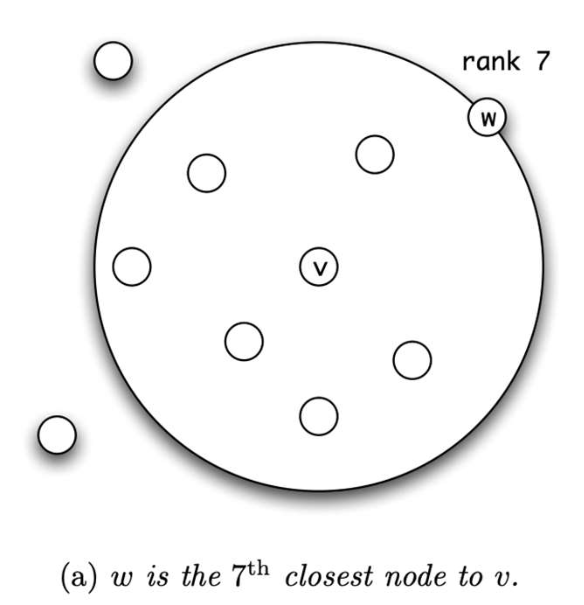
\includegraphics[width=0.7\linewidth]{screenshot005}
			\label{fig:screenshot005}
		\end{figure}
		In rank based friendship  with exponent $p$, $v$ creates a random link with $w$ proportional to $\mathrm{rank}(w)^{-p}$. If $w$ is at distance $d$ from $v$ then it is on the circumference of radius $d$ that contains $d^{2}$ closer nodes, therefore
		\begin{equation*}
			d^{-2}=\mathrm{rank}(w)^{-1}.
		\end{equation*}
		$p=1$ may be the right generalization. 
		For $p\approx 1$ the network is searchable. We can extend this to social foci defining the social distance $dist(v,w)$ between two people as the size of the smallest focus that includes both.\\
		In a one-dimensional ring we can track how long it taks for the message to reduce its distance by factors of 2 as it closes to the target.
		\begin{figure}[H]
			\centering
			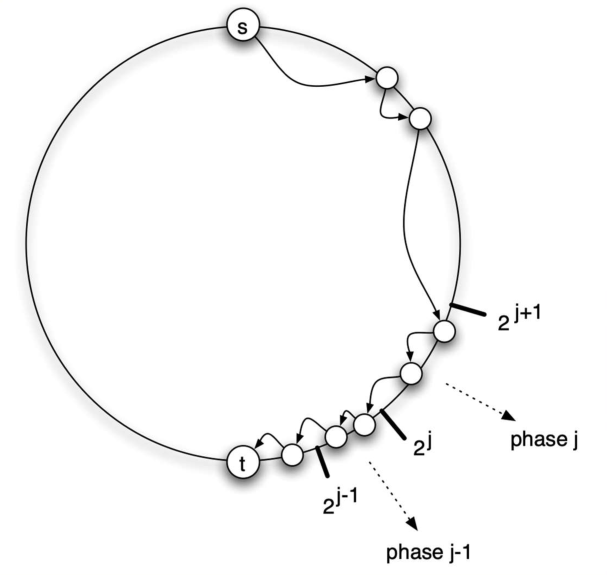
\includegraphics[width=0.7\linewidth]{screenshot006}
			\label{fig:screenshot006}
		\end{figure}
	\begin{riquadro}
		The message is in phase $j$ of the search if its distance from the target is between $2^{j}$ and $2^{j+1}$. We have a total of $\log_{2}n$ phases.
	\end{riquadro}
	We can write the total search time as the sum of times (number of steps) taken in each phase
	\begin{equation*}
		X=X_{1}+X_{2}+\ldots+X_{\log_{2}n}
	\end{equation*}
	so
	\begin{equation*}
		\ev{X}=\ev{X_{1}}+\ev{X_{2}}+\ldots+\ev{X_{\log_{2}n}}.
	\end{equation*}
	We want to show that $\forall j:\ev{X_{j}}\propto\log_{2}n$. The myopic seatch constructs a path that is exponentially smaller of then number of nodes. Here $v$ forms its long-range link to $w$ with probability proportional to $d(v,w)^{-1}$. We know the set of probabilities and we can set the missing constant of proportionality to $\frac{1}{Z}$ with $Z$ normalization constant $\sum_{u,v:u\neq v}d(u,v)^{-1}$. Notice that we have: 2 nodes at distance 1 from $v$, 2 nodes at distance 2, $\ldots$, 2 nodes
	at distance $\frac{n}{2}$
	:
	\begin{equation*}
		Z\leq2\left(1+\frac{1}{2}+\frac{1}{3}+\ldots+\frac{1}{\frac{n}{2}}\right)
	\end{equation*}
	but we know
	\begin{equation*}
		1+\frac{1}{2}+\frac{1}{3}+\ldots+\frac{1}{\frac{n}{2}}\leq 1+\int_{1}^{\frac{n}{2}}\frac{1}{x}\dx=1+\ln\left(\frac{n}{2}\right).
	\end{equation*}
	So
	\begin{equation*}
		Z\leq2+2\ln\left(\frac{n}{2}\right)
	\end{equation*}
	but $\ln x\leq\log_{2}x$ so
	\begin{equation*}
		Z\leq2+2\log_{2}\left(\frac{n}{2}\right)=2(\log_{2}n)
	\end{equation*}
	so the probability that $v$ links to $w$ is
	\begin{equation*}
		\frac{1}{Z}d(v,w)^{-1}\geq\frac{1}{2\log_{2}n}d(v,w)^{-1}.
	\end{equation*}
	The distance from target $t$ ends its phase $j$ when the distance is less than $2^{j}$. If ater the message has taken $v$'s long range contact we observe that distance to target will be reduced from $d$ to $\leq \frac{d}{n}$. 
	\begin{figure}[H]
		\centering
		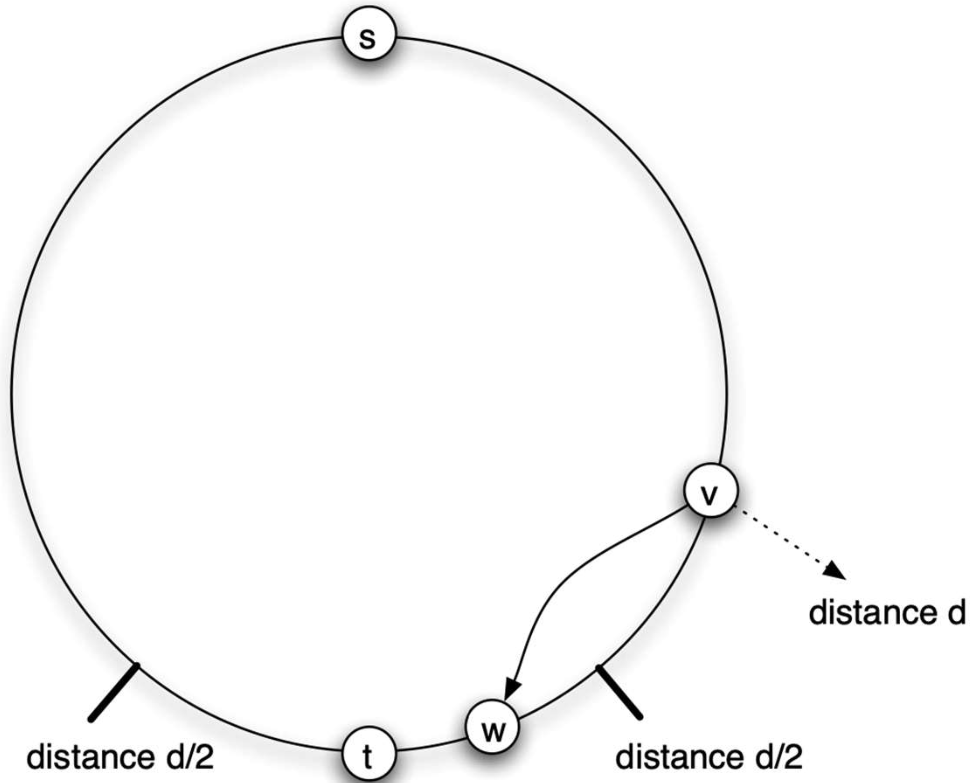
\includegraphics[width=0.7\linewidth]{screenshot007}
		\label{fig:screenshot007}
	\end{figure}
	Let $I$ be the set of nodes at distance $\leq\frac{d}{2}$ from $t$. $I$ has $d+1$ nodes (including $t$) and $\frac{d}{2}$ nodes on each sides. Each node $w$ in $I$:
	\begin{itemize}
		\item has distance at most $\frac{3d}{2}$ from $v$;
		\item has probability of being the long range contact of $v$ at least:
		\begin{align*}
			\frac{2}{2\log_{2}n}d(v,w)^{-1}&\geq\frac{1}{2\log_{2}n}\cdot\frac{1}{2\frac{d}{2}}\\
			&=\frac{1}{3d\cdot\log_{2}n}.
		\end{align*}
	\end{itemize}
	There are at most $d$ nodes in $I$, then the probability that one of them is the long-
	range contact of $v$ is at least:
	\begin{equation*}
		d\cdot\frac{1}{3d\cdot\log_{2}n}=\frac{1}{3\log_{2}n}.
	\end{equation*}
	This quantity does not depend on $d$. The probability that phase $j$ runs for at least $i$ steps is at most
	\begin{equation*}
		\left(1-\frac{1}{3\log_{2}n}\right)^{i-1}.
	\end{equation*}
	Since
	\begin{align*}
		\ev{X_{j}}&=1\cdot\pr\left(X_{j}=1\right)+2\cdot\pr\left(X_{j}=2\right)+\ldots\\
		&=\pr\left(X_{1}\geq 1\right)+\pr\left(X_{2}\geq 2\right)+\ldots
	\end{align*}
	we get
	\begin{equation*}
		\ev{X_{j}}\leq1+\left(1-\frac{1}{2\log_{2}n}\right)+\left(1-\frac{1}{2\log_{2}n}\right)^{2}++\left(1-\frac{1}{2\log_{2}n}\right)^{3}+\ldots
	\end{equation*}
	which converges to
	\begin{equation*}
		\frac{1}{1-\left(1-\frac{1}{3\log_{2}n}\right)}=3\log_{2}n.
	\end{equation*}
	So finally
	\begin{equation*}
		\ev{X}=\sum_{j}^{\log_{2}n}\ev{X_{j}}\leq3\left(\log_{2}n\right)^{2}.
	\end{equation*}
	\section{Epidemics}
	In the SIR model, we have
	\begin{equation*}
		R_{0}=\beta k.
	\end{equation*}
	The network of contacts is an infinite tree. The numbers of contacts is exactly $k$ with contagion probability of $\beta$. Let $q_{n}$ be the probability that the epidemic survives for at least $n$ waves and $q^{\star}=\lim_{n\to\infty}q_{n}$. We want to prove that 
	\begin{riquadro}
		if $R_{0}<1$ then $q^{\star}=0$; if $R_{0}>1$ then $q^{\star}>0$.
	\end{riquadro}
	The total umber of individuals at level $n$ is $k^{n}$. $X_{n}$ is a r.v. equal to the number of infected individuals at level $n$. For each individual $j$ at level $n$, $$Y_{nj}=\begin{cases}
	1&\text{if $j$ is infected}\\
	0&\text{otherwise}.
	\end{cases}$$
	So
	\begin{equation*}
		X_{n}=\sum_{j:1,\ldots,k^{n}}Y_{nj}
	\end{equation*}
	and
	\begin{equation*}
		\ev{X_{n}}=\ev{Y_{n1}}+\ldots+\ev{Y_{nk^{n}}}.
	\end{equation*}
	We have that
	\begin{equation*}
		\ev{Y_{nj}}=1\cdot\pr(Y_{nj}=1)+0\cdot\pr(Y_{nj}=0)=\pr(Y_{nj}=1).
	\end{equation*}
	So
	\begin{align*}
		\ev{X_{n}}&=\beta^{n}+\ldots+\beta^{n}\\
		&=k^{n}\beta^{n}\\
		&=(k\beta)^{n}=R^{n}_{0}.
	\end{align*}
	We can write the expectation as
	\begin{align*}
		\ev{X_{n}}&=1\cdot\pr(X_{n}=1)+2\cdot\pr(X_{n}=1)+3\cdot\pr(X_{n}=1)+\ldots\\
		&=\pr(X_{n}\geq1)+\pr(X_{n}\geq2)+\pr(X_{n}\geq3)+\ldots
	\end{align*}
	and for sure
	\begin{equation*}
		\ev{X_{n}}\geq\pr(X_{n}\geq1)
	\end{equation*}
	which is the probability that the epidemic survives after $n$ waves, hence $\pr(X_{n}\geq 1)=q_{n}$. Therefore since
	\begin{equation*}
		R_{0}<1\wedge\ev{X_{n}}=R^{n}_{0}\wedge \ev{X_{n}}\geq q_{n}
	\end{equation*}
	we have 
	\begin{equation*}
		\lim_{n\to\infty}R^{n}_{0}\implies\lim_{n\to\infty}q_{n}=0.
	\end{equation*}
	Define event $\star$: the disease spreads through the root's node first contact $j$ and then
	continues to persist down to $n$ levels in the part of the tree reachable through  $j$. So the root infects node $j$ with probability $\beta$ and goes through $n-1$ levels with probability $q_{n-1}$. Probability of event $\star$ is $\beta q_{n-1}$. Therefore, the disease fails to persist down to level n when all the $k$ copies of
	event $\star$ fail to hold. This happens with probability 
	\begin{equation*}
		(1-\beta q_{n-1})^{k}
	\end{equation*}
	but this is also probability $1-q_{n}$ that is the probability that the disease fails to persist to $n$ levels.
	\begin{equation*}
		1-q_{n}=(1-\beta q_{n-1})^{k}\iff q_{n}=1-(1-\beta q_{n-1})^{k}.
	\end{equation*}
	Assuming that the root is infected we have $q_{0}=1$ and we can build up all the values.\\
	To get the limiting value of the recursive $q_{n}=f(q_{n-1})$, we can study $f(x)=1-(1-\beta (x))^{k}$. We know that 
	\begin{equation*}
		f'(x)=\beta k(1-\beta x)^{k-1}\implies f'(x)>1\wedge f'(0)>f'(1).
	\end{equation*}
	We have $f'(0)=\beta k=R_{0}$. If $R_{0}>1$ then the slope of the tangent at $0$ is >1. We want to follow the sequence 
	\begin{equation*}
		1,f(1),f(f(1)),f(f(f(1))),\ldots
	\end{equation*}
	and we can track it down the bisector.
	\begin{figure}[H]
		\centering
		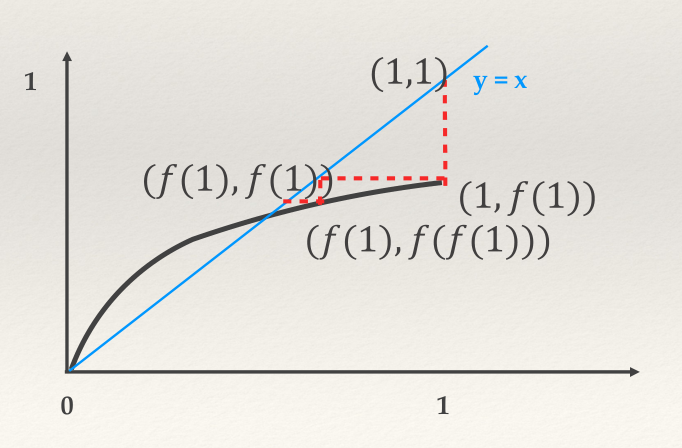
\includegraphics[width=0.7\linewidth]{screenshot008}
		\label{fig:screenshot008}
	\end{figure}
	The process converges to the point $(x^{\star},x^{\star})$ where the bisector intersects $y=f(x)$. The sequence $1,f(1),f(f(1)),f(f(f(1))),\ldots$ is the sequence $q_{0},q_{1},q_{1},\ldots$ and it converges to $x^{\star}>0$, the unique point at which $f(x)=x$. So
	\begin{equation*}
		R_{0}>1\implies\lim_{n\to\infty}q_{n}>0.
	\end{equation*}
	Also observe that if $R_{0}<1$ then the slope of the tangent at 0 is <1 so
	\begin{equation*}
		R_{0}<1\implies\lim_{n\to\infty}q_{n}=0.
	\end{equation*}
	Recall the heterogeneity parameter
	\begin{equation*}
		\kappa=\frac{\langle k^{2}\rangle}{\langle k\rangle^{2}}.
	\end{equation*}
	In random networks $\kappa\approx 1$, if the distribution is heterogeneous $\kappa\gg1$. The degree distribution is approximated by a power law
	\begin{equation*}
		p_{k}\propto k^{-\gamma}
	\end{equation*}
	with $2<\gamma\leq 3$ then $\langle k^{2}\rangle\to\infty$. Define as $s(t)$, $i(t)$ and $r(t)$ as the fraction of S, I and R individuals at time $t$. The initial conditions with only one infect at $t=0$ are
	\begin{equation*}
		\begin{array}{c}
			i(0)=\frac{1}{N}\\
			s(0)=1-i(0)\\
			r(0)=0.
		\end{array}
	\end{equation*}
	The infected node transmits the disease with probability $\beta:i+s\xrightarrow{\beta}i+i$.
	\begin{riquadro}[Fully mixed hypothesis]
		an infected individual comes into contact with other $\langle k\rangle s(t)$
		susceptible individuals in a unit time. 
	\end{riquadro}
	\subsection{No recovery: SI}
	This means that the new infections $\dif i(t)$ during a time $\dt$ is
	\begin{equation*}
		\dif i(t)=\beta\langle k\rangle s(t)i(t)\dt.
	\end{equation*}
	and since $s(t)=1-i(t)$ we get
	\begin{equation*}
		\frac{\dif i}{\dt}=\beta\langle k\rangle i(1-i)\implies\frac{\dif i}{i}+\frac{\dif i}{1-i}=\beta\langle k\rangle\dt.
	\end{equation*}
	Integrating both sides yields
	\begin{equation*}
		\ln i-\ln(1-i)+C=\beta\langle k\rangle t.
	\end{equation*}
	From an initial condition $i_{0}=i(0)$ we get $C$:
	\begin{equation*}
		C=\ln(1-i_{0})-\ln i_{0}.
	\end{equation*}
	So
	\begin{equation*}
			\begin{array}{>{\displaystyle}c}
				\ln i-\ln(1-i)+\ln(1-i_{0})-\ln i_{0}=\beta\langle k\rangle t\\
				\Downarrow\\
				i=\frac{i_{0}e^{\beta\ang{k}t}}{1-i_{0}+i_{0}e^{\beta\ang{k}{t}}}
			\end{array}
	\end{equation*}
	which is the logistic curve.
	\subsection{Recovery: SIS}
	Individuals recover with rate $\mu:i\xrightarrow{\mu}s$. Is there a threshold for $R_{0}=\frac{\beta\ang{k}}{\mu}$? We now have
	\begin{equation*}
		\frac{\dif i}{\dt}=\beta\ang{k}i(1-i)-\mu i
	\end{equation*}
	which is solved by
	\begin{equation*}
		i=\left(1-\frac{\mu}{\beta\ang{k}}\right)\frac{Ce^{(\beta\ang{k}-\mu)t}}{1+Ce^{\left(\beta\ang{k}-\mu\right)t}}.
	\end{equation*}
	With initial condition $i_{0}=i(0)$ we have
	\begin{equation*}
		C=\frac{i_{0}}{1-i_{0}-\frac{\mu}{\beta\ang{k}}}.
	\end{equation*}
	\begin{itemize}
		\item If $R_{0}>1\implies \beta\ang{k}>\mu$, then $\lim_{t\to\infty}i(t)=1-\frac{\mu}{\beta\ang{k}}$.
		\item If $R_{0}<1\implies \beta\ang{k}<\mu$, then $\lim_{t\to\infty}i(t)=0$.
	\end{itemize}
	\subsection{Recovery and resistance: SIR}
	Individuals recover with rate $\mu:i\xrightarrow{\mu}r$. Is there a threshold for $R_{0}=\frac{\beta\ang{k}}{\mu}$? We have
	\begin{align*}
		\frac{\dif s}{\dt}&=-\beta\ang{k}is=-\beta\ang{k}i(1-r-i)\\
		\frac{\dif i}{\dt}&=\beta\ang{k}i(1-r-i)-\mu i\\
		\frac{\dif r}{\dt}&=\mu i.
	\end{align*}
	The boundaries conditions are 
	\begin{equation*}
		\begin{array}{l}
			s+r+i=1\\
			s(0)=s_{0}\\
			r(0)=r_{0}\\
			i(0)=i_{0}=1-s_{0}.
		\end{array}
	\end{equation*}
	To compute the asymptotic value of $r$ we have that
	\begin{align*}
		\frac{\dif r}{\dt}&=\mu\left(1-r-s_{0}e^{-R_{0}r}\right)=0\\
		&\implies r=1-s_{0}e^{-R_{0}r}.
	\end{align*}
	For large networks with $N\to\infty$ we have $s_0\approx 1$ so $r=1-e^{-R_{0}r}$ so
	\begin{itemize}
		\item if $R_{0}>1$ then $\lim_{t\to\infty}r=1$;
		\item if $R_{0}<1$ then $\lim_{t\to\infty}r=0$.
	\end{itemize}
	We have
	\begin{equation*}
		\frac{\dif s}{\dt}=-\beta\ang{k}si\implies i=-\frac{i}{\beta\ang{k}s}\frac{\dif s}{\dt}
	\end{equation*}
	and
	\begin{equation*}
		\frac{\dif r}{\dt}=\mu i\implies i=\frac{1}{\mu}\frac{\dif r}{\dt}
	\end{equation*}
	so putting them together we have
	\begin{align*}
		&\frac{1}{\mu}\frac{\dif r}{\dt}=-\frac{1}{\beta\ang{k}s}\frac{\dif s}{\dt}\\
		\implies&\frac{\beta\ang{k}}{\mu}\frac{\dif r}{\dt}=-\frac{1}{s}\frac{\dif s}{\dt}\\
		\implies&\frac{1}{2}\frac{\dif s}{\dt}=-R_{0}\frac{\dif r}{\dt}\\
		\implies&\ln s=-R_{0}r+C \\
		\implies&\ln s=-R_{0}r+\ln s_{0}\\
		\implies&s=s_{0}e^{-R_{0}r}
	\end{align*}
	but since $s+r+i=1$ and $\frac{\dif r}{\dt}=\mu i$ we have
	\begin{equation*}
		\frac{\dif r}{\dt}=\mu\left(1-r-s_{0}e^{-R_{0}r}\right).
	\end{equation*}
	\begin{riquadro}[Degree-block approximation]
		Assumes nodes with the same degree are statistically equivalent. $i_{k}=\frac{I_{k}}{N_{k}}$ is the fraction of nodes with degree $k$ that are infected among all $N_{k}$ degree-$k$ nodes in the network. The total fraction of infected nodes can be calculated as it follows:
		\begin{equation*}
			i=\sum_kp_ki_k.
		\end{equation*}
	\end{riquadro}
	\subsection{SI model on a network}
	Each degree $k$ has its equation
	\begin{equation*}
		\frac{\dif i_{k}}{\dt}=\beta(1-i_{k})k\Theta_{k}.
	\end{equation*}
	We do not use the average $k$ anymore but we have the density function $\Theta_k$ (fraction of infected neighbours of a susceptible node with degree $k$). If $i_{k}$ is small:
	\begin{equation*}
		\frac{\dif i_{k}}{\dt}\approx\beta k\Theta_{k}.
	\end{equation*}
	$\Theta_{k}$ is independent of $k$:
	\begin{equation*}
		\Theta_{k}\approx i_{0}\frac{\ang{k}-1}{\ang{k}}e^{\frac{1}{\tau}}\qquad\text{with }\tau=\frac{\ang{k}}{\beta\left(\ang{k^{2}}-\ang{k}\right)}.
	\end{equation*}
	$\tau$ is the characteristic time of spread. 
	\begin{align*}
		&\frac{\dif i_{k}}{\dt}\approx\beta ki_{0}\frac{\ang{k}-1}{\ang{k}}e^{\frac{1}{\tau}}\\
		\implies&i_{k}=i_{0}\left(1+\frac{k\ang{k}-1}{\ang{k^{2}}-\ang{k}}\left(e^{\frac{1}{\tau}}-1\right)\right).
	\end{align*}
	The higher the degree of a node, the more likely it is to become infected. We can write
	\begin{equation*}
		i_{k}=g(t)+kf(t)
	\end{equation*}
	and calculate the total fraction of infected nodes
	\begin{align*}
		i&=\int_{0}^{k_{\max}}i_{k}p_{k}\dif k\\
		&=i_{0}\left(1+\frac{\ang{k}^{2}-\ang{k}}{\ang{k^{2}}-\ang{k}}\left(e^{\frac{1}{\tau}-1}\right)\right).
	\end{align*}
	We have that the characteristic time $\tau=\frac{\ang{k}}{\beta\left(\ang{k^{2}}-\ang{k}\right)}$:
	\begin{itemize}
		\item in random networks (where $\kappa=\frac{\ang{k^{2}}}{\ang{k}^{2}}\approx 1\implies\ang{k^{2}}\approx\ang{k}^{2}$) is $\tau\approx\frac{1}{\beta\ang{k}}$;
		\item in heterogeneous networks (where $\kappa\gg1\implies\ang{k^{2}}\gg\ang{k}^{2}$) is $\tau\ll\frac{1}{\beta\ang{k}}$;
		\item in scale-free networks (where $\ang{k^{2}}\xrightarrow{N\to\infty}\infty$) is $\tau\to0$.
	\end{itemize}
	\subsection{SIS model on a network}
	Here the continuum equation is
	\begin{equation*}
		\frac{\dif i_{k}}{\dt}=\beta\left(1-i_{k}\right)k\Theta_{k}(t)-\mu i_{k}.
	\end{equation*}
	The characteristic time becomes
	\begin{equation*}
		\tau=\frac{\ang{k}}{\beta\ang{k^{2}}-\mu\ang{k}}.
	\end{equation*}
	Define the spreading rate $\lambda=\frac{\beta}{\mu}$ which gives us $R_{0}=\lambda\ang{k}$. We want to look for the epidemic threshold $\lambda_{c}$ (the pathogen can spread if $\lambda>\lambda_{c}$). This means finding $\tau>0$.
	\begin{align*}
		\tau>0&\implies\frac{\ang{k}}{\beta\ang{k^{2}}-\mu\ang{k}}>0\\
		&\implies \beta\ang{k^{2}}>\mu\ang{k}\\
		&\implies\lambda=\frac{\beta}{\mu}>\frac{\ang{k}}{\ang{k^{2}}}\\
		&\implies\lambda_{c}=\frac{\ang{k}}{\ang{k^{2}}}.
	\end{align*}
	\begin{itemize}
		\item In random networks we have $\ang{k^{2}}\approx\ang{k}$ so $\lambda_{c}\approx\frac{1}{\ang{k}}$.
		\item In heterogeneous networks we have $\ang{k^{2}}\gg\ang{k}^{2}$ so $\lambda_{c}$ is expected to vanish for increasingly homogeneous networks.
		\item In scale-free networks (where $\ang{k^{2}}\xrightarrow{N\to\infty}\infty$) we have $\lambda_{c}=0$.
	\end{itemize}
	\subsection{Random immunization}
	We need to monitor $\lambda$. Let's assume the pathogen follows the SIS model: a random fraction of individuals $g$ is immunized. The effective degree of each susceptible node goes from $\ang{k}$ to $\ang{k}(1-g)$ and the spreading rate becomes $\lambda'=\lambda(1-g)$. For a high $g_{c}$ $\lambda'$ may fall below the epidemic threshold $\lambda_{c}$. On a random network:
	\begin{align*}
	&	\lambda_{c}=\lambda(1-g_{c})=(1-g_{c})\frac{\beta}{\mu}\approx\frac{1}{\ang{k}}\\
	\implies&g_{c}\approx1-\frac{\mu}{\beta\ang{k}}.
	\end{align*}
	On a network with $\kappa\gg1$:
	\begin{align*}
		&	\lambda_{c}=\lambda(1-g_{c})=(1-g_{c})\frac{\beta}{\mu}\approx\frac{\ang{k}}{\ang{k^{2}}}\\
		\implies&g_{c}\approx1-\frac{\mu\ang{k}}{\beta\ang{k^{2}}}.
	\end{align*}
	In scale-free networks $g_{c}=1$. In the real world random immunization is inefficient because of vanishing epidemic threshold.
	\begin{riquadro}[Friendship paradox]
		\begin{itemize}
			\item Group 0: a random fraction of nodes $p$.
			\item Group 1: select randomly a link from each node in group 0. We stop at the set of nodes to which these links connect to.
			\item Immunize group 1.
		\end{itemize}
	\end{riquadro}
	\subsection{Forecasts and prevention}
	\begin{riquadro}[GLEAM]
		Network-based computational model. It maps each geographic location into the nodes of a network: transport is provided by global transportation data (``schedules'') and it estimates the epidemic parameters relying on chronological data.
	\end{riquadro}
	\end{multicols*}
\end{document}